%%%%%%%%%%%%%%%%%%%%%%%%%%%%%%%%%%%%%%%%%%%%%%%%%%%%%%%%%%%%%%%%%%%%%%%%%%%%%%%%%%
\begin{frame}[fragile]\frametitle{}
\begin{center}
{\Large Modern RL}
\end{center}
\end{frame}

%%%%%%%%%%%%%%%%%%%%%%%%%%%%%%%%%%%%%%%%%%%%%%%%%%%%%%%%%%%%%%%%%%%%%%%%%%%%%%%%%%
\begin{frame}[fragile]\frametitle{}
\begin{center}
{\Large Curiosity}
\end{center}
\end{frame}

%%%%%%%%%%%%%%%%%%%%%%%%%%%%%%%%%%%%%%%%%%%%%%%%%%%%%%%%%%%%%%%%%%%%%%%%%%%%%%%%%%
\begin{frame}[fragile]\frametitle{Reinforce (Problems)}

Two Major Problems in Modern RL

\begin{itemize}
\item Sparse rewards or non-existing rewards problem: that is, most rewards do not contain information, and hence are set to zero. However, as rewards act as feedback for RL agents, if they don’t receive any, their knowledge of which action is appropriate (or not) cannot change. For instance, in Vizdoom “DoomMyWayHome,” your agent is only rewarded if it finds the vest. However, the vest is far away from your starting point, so most of your rewards will be zero.
\item Extrinsic reward function is handmade — that is, in each environment, a human has to implement a reward function. But how we can scale that in big and complex environments?
\item Therefore, a solution to these problems is to develop a reward function that is intrinsic to the agent, i.e., generated by the agent itself. 
\end{itemize}

{\tiny (Ref: Curiosity-Driven Learning through Next State Prediction - Thomas Simonini)}

\end{frame}

%%%%%%%%%%%%%%%%%%%%%%%%%%%%%%%%%%%%%%%%%%%%%%%%%%%%%%%%%%%%%%%%%%%%%%%%%%%%%%%%%%
\begin{frame}[fragile]\frametitle{Curiosity}
Curiosity-Driven Learning through Next State Prediction

% \begin{center}
% 
\includegraphics[width=0.4\linewidth,keepaspectratio]{rl59}
% \end{center}

\begin{itemize}
\item MThe idea of curiosity-driven learning is to build a reward function that is intrinsic to the agent (that is generated by the agent itself). In this sense, the agent will act as a self-learner since it will be the student, but also its own feedback master.
\item This intrinsic reward mechanism is known as curiosity because it explores states that are novel/unfamiliar. In order to achieve that, our agent will receive a high reward when exploring new trajectories.
\item This reward design is based on how human plays — some suppose we have an intrinsic desire to explore environments and discover new things! There are different ways to calculate this intrinsic reward, and we’ll focus on this article on curiosity through next-state prediction.
\end{itemize}

{\tiny (Ref: Curiosity-Driven Learning through Next State Prediction - Thomas Simonini)}


\end{frame}


%%%%%%%%%%%%%%%%%%%%%%%%%%%%%%%%%%%%%%%%%%%%%%%%%%%%%%%%%%%%%%%%%%%%%%%%%%%%%%%%%%
\begin{frame}[fragile]\frametitle{Super Mario Bros}
Curiosity-Driven Learning through Next State Prediction

\begin{center}
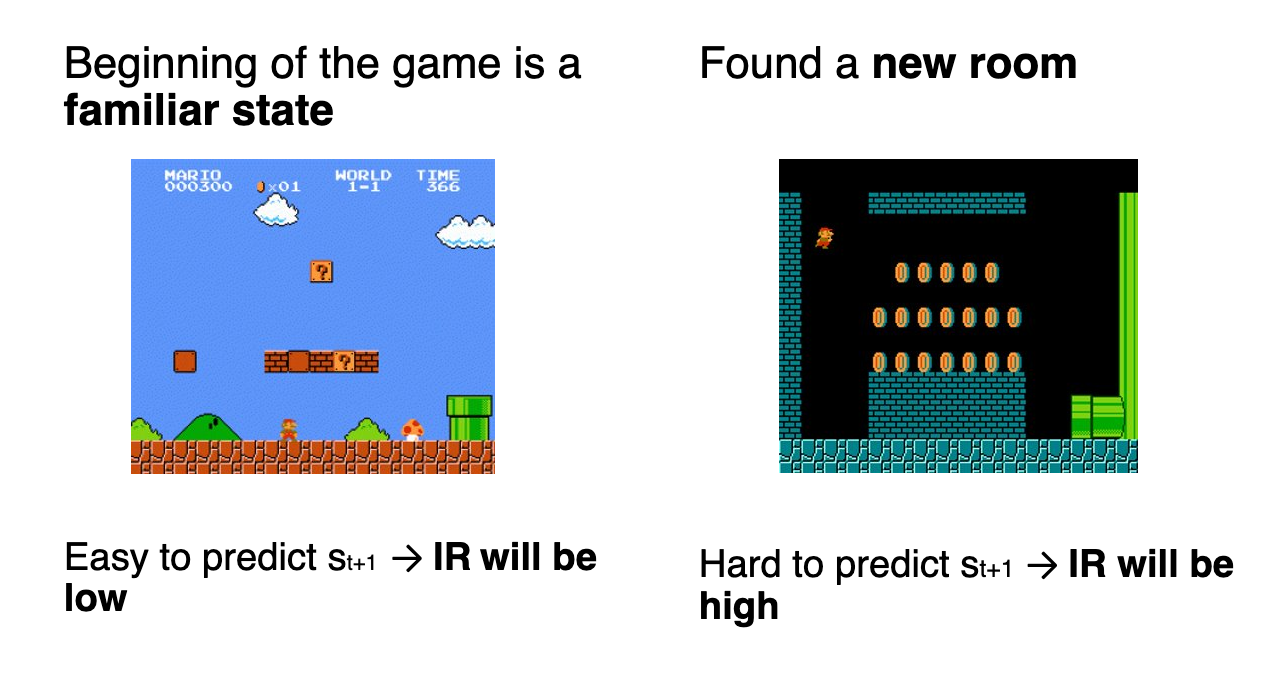
\includegraphics[width=0.6\linewidth,keepaspectratio]{rl130}
\end{center}

\begin{itemize}
\item If you spend a lot of time in the beginning of the game (which is not new), the agent will be able to accurately predict what the next state will be, so the reward will be low.
\item  On the other hand, if you discover a new room, our agent will be very bad in predicting the next state, so the agent will be pushed to explore this room.
\end{itemize}

{\tiny (Ref: Curiosity-Driven Learning through Next State Prediction - Thomas Simonini)}


\end{frame}

%%%%%%%%%%%%%%%%%%%%%%%%%%%%%%%%%%%%%%%%%%%%%%%%%%%%%%%%%%%%%%%%%%%%%%%%%%%%%%%%%%
\begin{frame}[fragile]\frametitle{Super Mario Bros}


\begin{itemize}
\item Consequently, measuring error requires building a model of environmental dynamics that predicts the next state given the current state and the action. The question that we can ask here is: how we can calculate this error?
\item But we can’t predict $s_{t+1}$ by predicting the next frame as we usually do. Why?
\item First, because it’s hard to build a model that is able to predict high-dimension continuous state space, such as an image. It’s hard to predict the pixels directly, but now imagine you’re in Doom, and you move left — you need to predict 248*248 = 61504 pixels!
\end{itemize}

{\tiny (Ref: Curiosity-Driven Learning through Next State Prediction - Thomas Simonini)}


\end{frame}

%%%%%%%%%%%%%%%%%%%%%%%%%%%%%%%%%%%%%%%%%%%%%%%%%%%%%%%%%%%%%%%%%%%%%%%%%%%%%%%%%%
\begin{frame}[fragile]\frametitle{Super Mario Bros}


It means that in order to generate curiosity, we can’t predict the pixels directly and need to use a better feature representation by projecting the raw pixels space into a feature space that will hopefully only keep the relevant information elements that can be leveraged by our agent.


\begin{center}
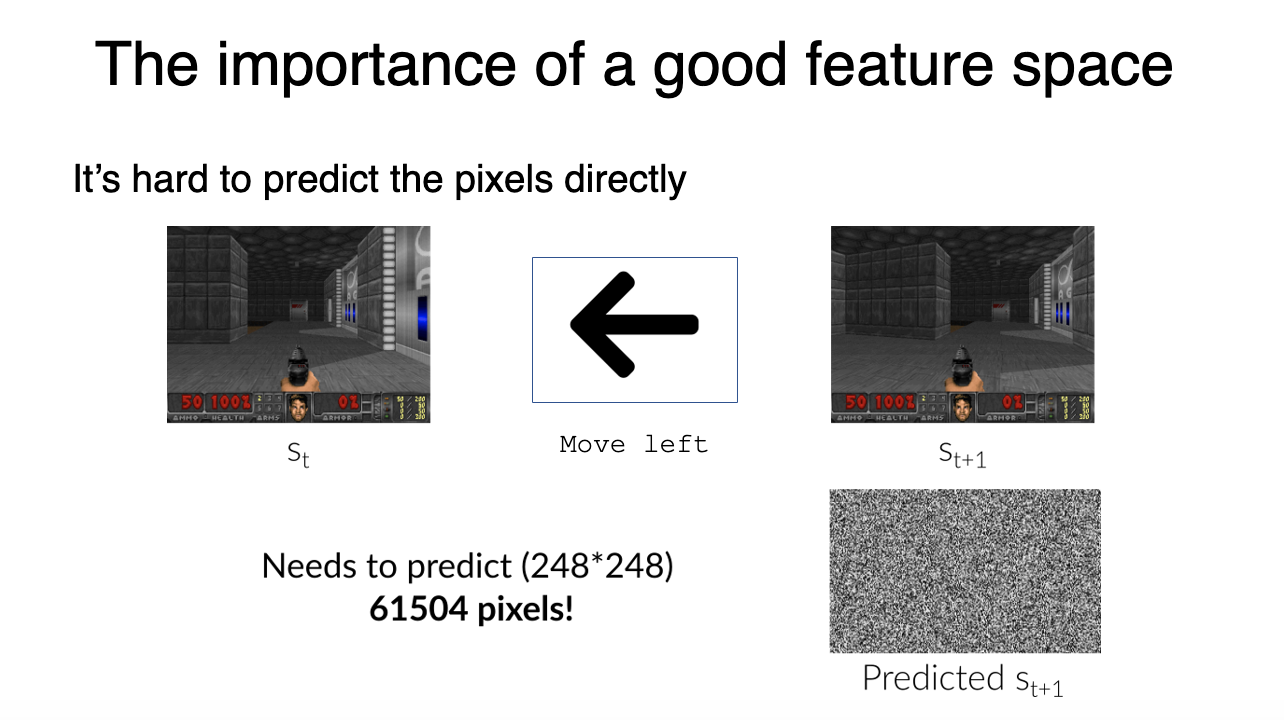
\includegraphics[width=0.8\linewidth,keepaspectratio]{rl131}
\end{center}

{\tiny (Ref: Curiosity-Driven Learning through Next State Prediction - Thomas Simonini)}


\end{frame}

%%%%%%%%%%%%%%%%%%%%%%%%%%%%%%%%%%%%%%%%%%%%%%%%%%%%%%%%%%%%%%%%%%%%%%%%%%%%%%%%%%
\begin{frame}[fragile]\frametitle{Super Mario Bros}

Three rules are defined in the original paper for a good representation feature space:

\begin{itemize}
\item Model things that can be controlled by the agent.
\item Model things that can’t be controlled by the agent but can affect the agent.
\item Don’t model things that are not controlled by the agent and have no effect on it.
\end{itemize}

The second reason we can’t predict $s_{t+1}$ by predicting the next frame as we usually do? It might just not be the right thing to do:

{\tiny (Ref: Curiosity-Driven Learning through Next State Prediction - Thomas Simonini)}


\end{frame}

%%%%%%%%%%%%%%%%%%%%%%%%%%%%%%%%%%%%%%%%%%%%%%%%%%%%%%%%%%%%%%%%%%%%%%%%%%%%%%%%%%
\begin{frame}[fragile]\frametitle{Car}



\begin{itemize}
\item Imagine you need to study the movement of the tree leaves in a breeze. First of all, it’s already hard enough to model breeze, so predicting the pixel location of each leaves at each time step is even harder.
\item So instead of making predictions in the raw sensory space (pixels), we need to transform the raw sensory input (array of pixels) into a feature space with only relevant information.
\item Let’s take this example: your agent is a self driving car. If we want to create a good feature representation, we need to model:
\end{itemize}

\begin{center}
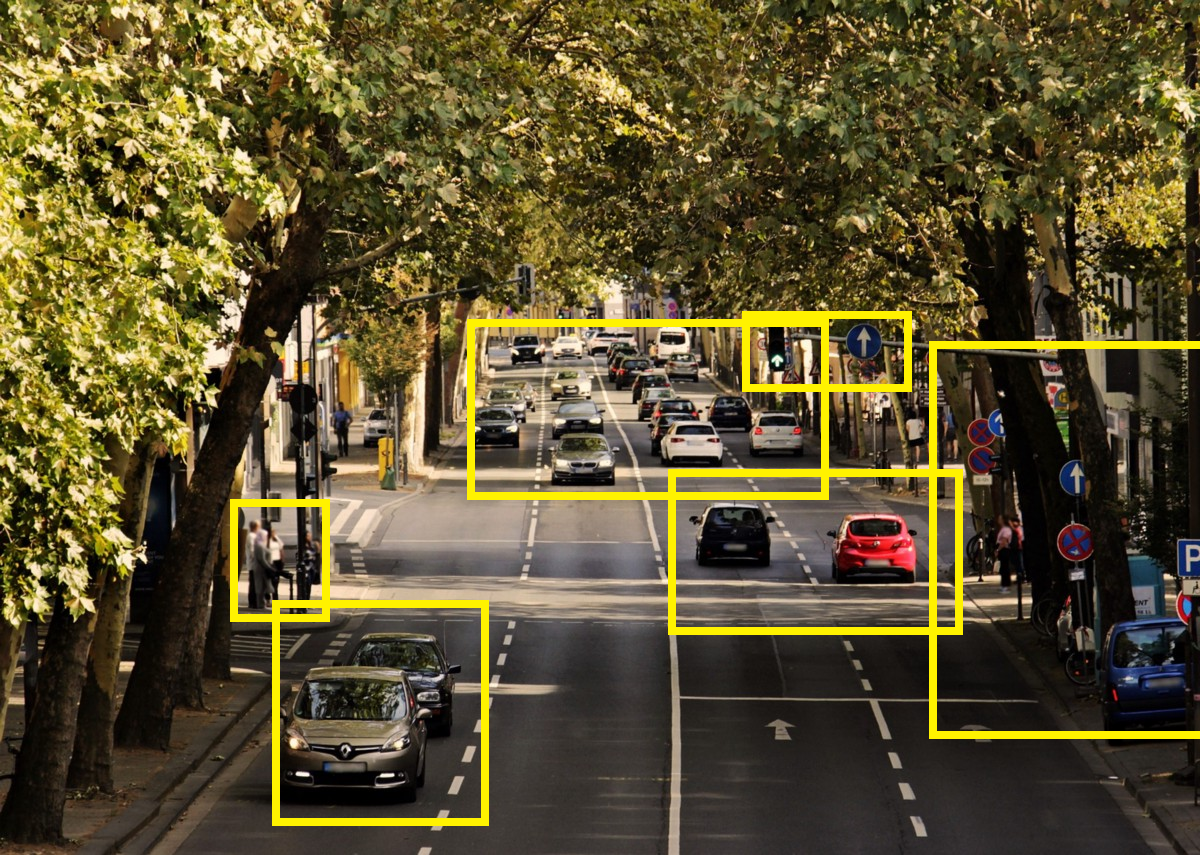
\includegraphics[width=0.4\linewidth,keepaspectratio]{rl132}
\end{center}


{\tiny (Ref: Curiosity-Driven Learning through Next State Prediction - Thomas Simonini)}


\end{frame}

%%%%%%%%%%%%%%%%%%%%%%%%%%%%%%%%%%%%%%%%%%%%%%%%%%%%%%%%%%%%%%%%%%%%%%%%%%%%%%%%%%
\begin{frame}[fragile]\frametitle{Feature Representation}

A good feature representation would be our car (controlled by our agent) and the other cars (we can’t control it, but that can affect the agent), but we don’t need to model the leaves (it doesn’t affect the agent, and we can’t control it). By only keeping this information, we will have a feature representation with less noise.

The desired embedding space should:

\begin{itemize}
\item Be compact in terms of dimensional (remove irrelevant parts of the observation space).
\item Preserve sufficient information about the observation.
\item Be stable, because non-stationary rewards (rewards that decrease through time since curiosity decreases through time) make it difficult for reinforcement agents to learn.
\end{itemize}

In order to calculate the predicted next state and the real feature representation of the next state, we can use an Intrinsic Curiosity Module (ICM).

{\tiny (Ref: Curiosity-Driven Learning through Next State Prediction - Thomas Simonini)}


\end{frame}

%%%%%%%%%%%%%%%%%%%%%%%%%%%%%%%%%%%%%%%%%%%%%%%%%%%%%%%%%%%%%%%%%%%%%%%%%%%%%%%%%%
\begin{frame}[fragile]\frametitle{ICM Module}

The ICM Module is the system that helps us to generate curiosity. It’s composed of two neural networks; each of them has an important task.

\begin{center}
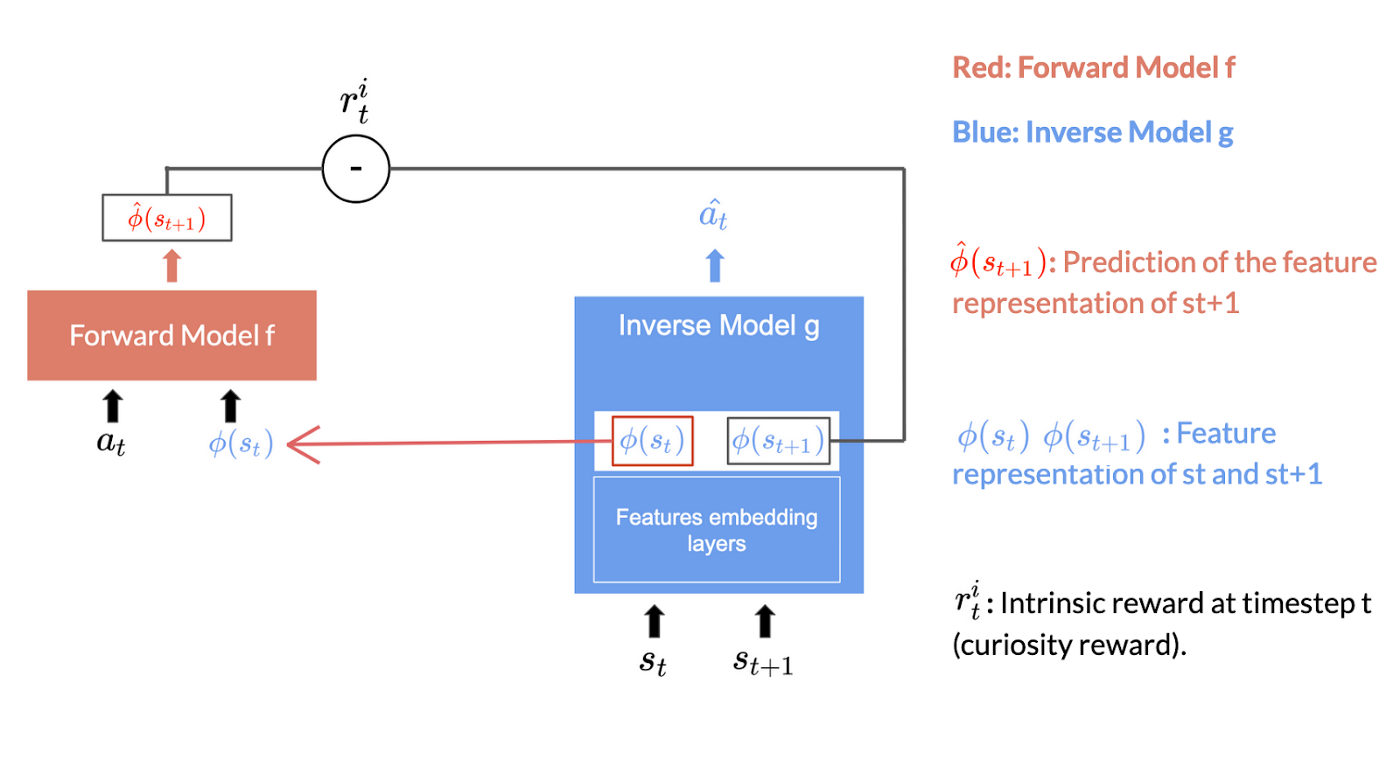
\includegraphics[width=\linewidth,keepaspectratio]{rl133}
\end{center}


{\tiny (Ref: Curiosity-Driven Learning through Next State Prediction - Thomas Simonini)}


\end{frame}

%%%%%%%%%%%%%%%%%%%%%%%%%%%%%%%%%%%%%%%%%%%%%%%%%%%%%%%%%%%%%%%%%%%%%%%%%%%%%%%%%%
\begin{frame}[fragile]\frametitle{The Inverse Model}

The Inverse Model (g), aims at predicting the action $a(t)$, and in doing so, it learns an internal feature representation of the state and next state, denoted by $\phi(s(t))$ and $\phi(s(t+1))$.
\begin{center}
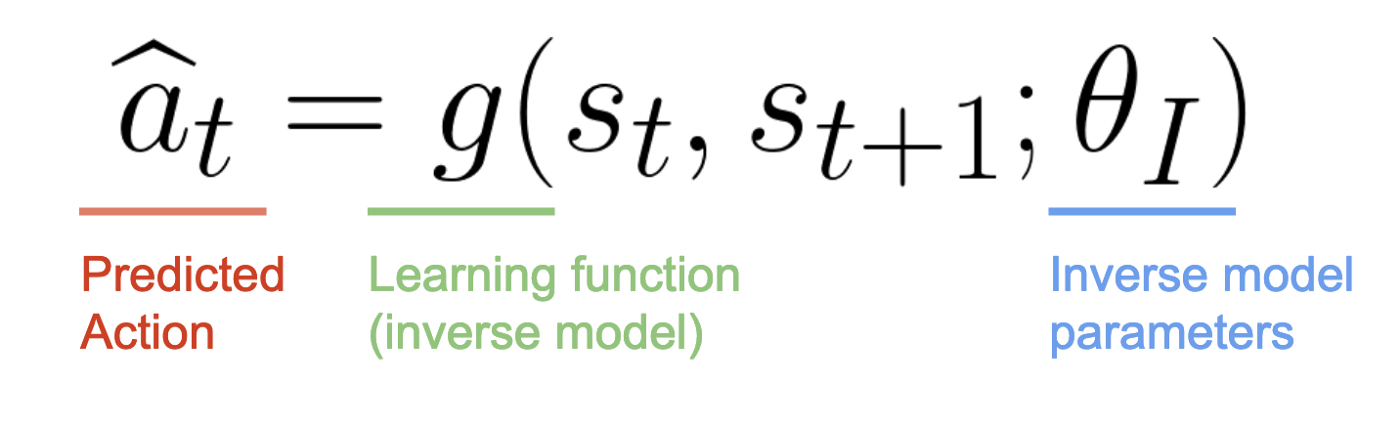
\includegraphics[width=0.6\linewidth,keepaspectratio]{rl134}
\end{center}

Since this neural network is only used to predict the action, it has no incentive to represent within its feature embedding space the factors of variation in an environment that does not affect the agent itself.


{\tiny (Ref: Curiosity-Driven Learning through Next State Prediction - Thomas Simonini)}


\end{frame}

%%%%%%%%%%%%%%%%%%%%%%%%%%%%%%%%%%%%%%%%%%%%%%%%%%%%%%%%%%%%%%%%%%%%%%%%%%%%%%%%%%
\begin{frame}[fragile]\frametitle{The Inverse Model}

Lastly, the inverse model loss is given by the cross entropy between our predicted action â(t) and the real action a(t):


\begin{center}
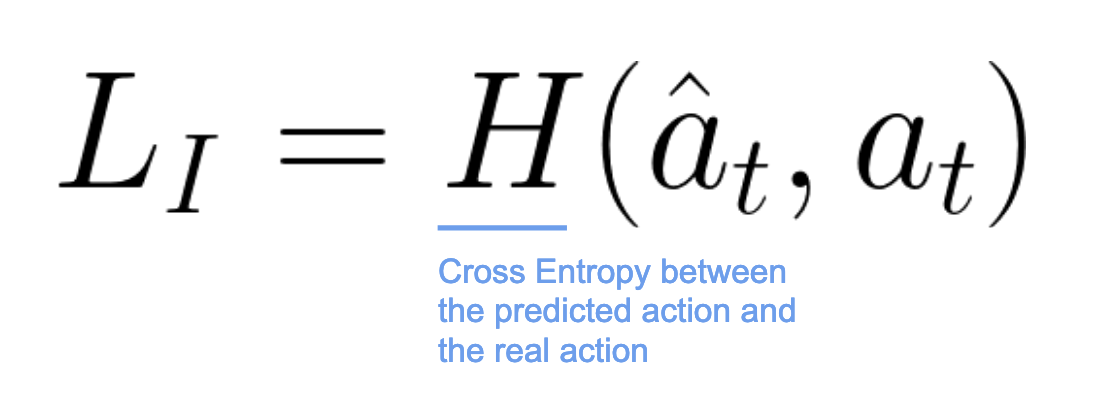
\includegraphics[width=0.4\linewidth,keepaspectratio]{rl135}
\end{center}



{\tiny (Ref: Curiosity-Driven Learning through Next State Prediction - Thomas Simonini)}


\end{frame}

%%%%%%%%%%%%%%%%%%%%%%%%%%%%%%%%%%%%%%%%%%%%%%%%%%%%%%%%%%%%%%%%%%%%%%%%%%%%%%%%%%
\begin{frame}[fragile]\frametitle{The Forward model}

The Forward Model (f), predicts the feature representation of next state $\phi(s(t+1))$ given $\phi(s(t))$ and $a(t)$.

\begin{center}
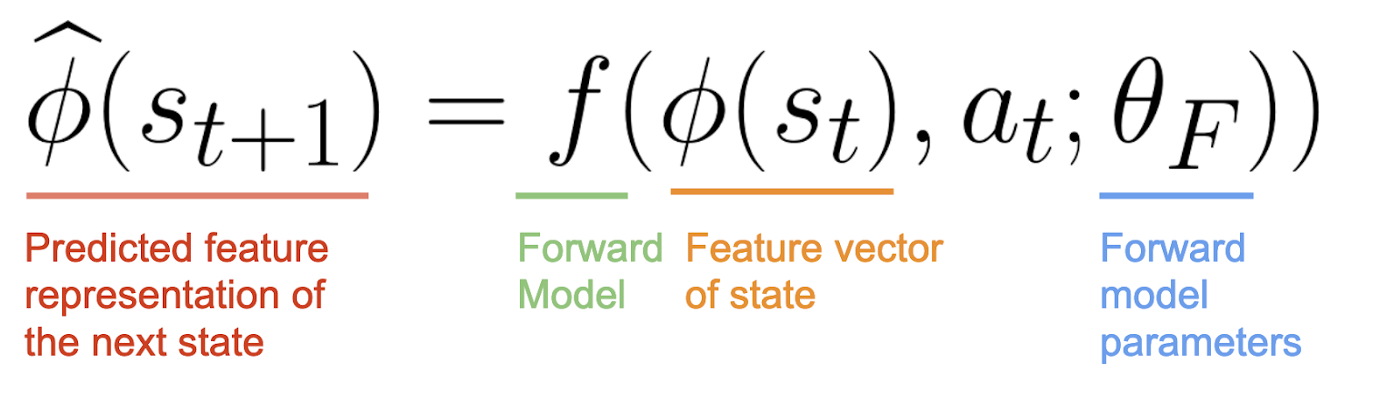
\includegraphics[width=0.6\linewidth,keepaspectratio]{rl136}
\end{center}

Consequently, curiosity will be a real number, i.e., the L2 normed difference between our predicted feature vector of the next state

Finally, the overall optimization problem of this module is a composition of Inverse Loss and Forward Loss.

And we provide the prediction error of the forward dynamics model to the agent as an intrinsic reward to encourage its curiosity.

{\tiny (Ref: Curiosity-Driven Learning through Next State Prediction - Thomas Simonini)}


\end{frame}


%%%%%%%%%%%%%%%%%%%%%%%%%%%%%%%%%%%%%%%%%%%%%%%%%%%%%%%%%%%%%%%%%%%%%%%%%%%%%%%%%%
\begin{frame}[fragile]\frametitle{}
\begin{center}
{\Large Advantage Actor Critic (A2C)}
\end{center}

TBD : https://huggingface.co/blog/deep-rl-a2c
\end{frame}


%%%%%%%%%%%%%%%%%%%%%%%%%%%%%%%%%%%%%%%%%%%%%%%%%%%%%%%%%%%%%%%%%%%%%%%%%%%%%%%%%%
\begin{frame}[fragile]\frametitle{}
\begin{center}
{\Large Proximal Policy Optimization (PPO)}
\end{center}

TBD : https://huggingface.co/blog/deep-rl-ppo

\end{frame}



